\documentclass[mim_thesis.tex]{subfiles} 
\begin{document}
Since the start of openEHR CKM operation, a huge percentage of archetypes have been created. Many contributors have developed them around the world. With this, a lot of changes can be made to the root lining, and to not allow a divergence in the content of each created archetype, the openEHR group defined rules and methodologies for the archetype development process, commonly called Archetype Development Life Cycle (ADLC) \citep{Madsen2010}, which is based on the Software Development Life Cycle (SDLC). This process will be explained in detail in this chapter.


\section{The Archetype Development Process}
The steps for the process of an achetype development process start at the identifications of all the clinical requirements, searching if compatible or reusable archetypes exists in the openEHR CKM, if not, build the archetypes and then submit them to the openEHR CKM repository, where a process of archetype review will be made. In case of common consensus by the editors of the repository, the archetype will be published. Inside of all these steps, there are other sub-processes that needs to be done. M. Madsen in 2010 proposed the phases of an archetype development process. They are composed by:

\begin{enumerate}[noitemsep]
\item \textbf{Planning phase} - containing the content gathering and clinical engagement;
\item \textbf{Analysis phase} - data analysis and consolidation, draft modeling estimate and knowledge of current available archetypes;
\item \textbf{Requirements specification phase} - where are presented the clarifications of content questions and other issues with end users and start of a modeling plan creation;
\item \textbf{Design phase} - including the archetype design, creation of clinical models and the addition of terminology;
\item \textbf{Testing, evaluation and review phase} - review of interactions between content and terminology and modeling review;
\item \textbf{Delivery phase} - model sign-off and hand over to vendor;
\item \textbf{Maintenance phase} - fixing small issues that can appear and giving correction updates if required.
\end{enumerate}

In the first phase of the development process is necessary to define essential procedures for analysis and choose a work group (project manager, a clinical expert/ physician, terminology and technical expert and an openEHR modeler) \citep{moner2018archetype}. Usually, this is the crucial point that will allow to do not waste time and money on reviewing all the procedures in every step of development, in case of wrong initial analysis. When making an initial data analysis, is mandatory to understand and determine all the necessary initial requirements, data collection and content gathering. This can be done by analyzing the many possible sources, like the paper based forms used on the health care institutions by the physicians, understanding how the work flow is processed in these institutions and which guidelines have been used. To identify the different clinical concepts, the creation of a mindmap could help to visualize the gathered data during this process stage \citep{marcos2010towards}. Also, checking how the existing electronic health records present the forms and the information stored on their databases can help. All the collected information can result in a archetype that will be fitting the main purpose. Nevertheless, include all the external parties and end-users involved in the process to have basic training on the openEHR methodology should optimize the content gathering process. When the first step is almost concluded, is necessary to start a modeling process plan, which allows to have an idea of what the next process of archetype development will look like. It is always vital to have collaborative meetings to discuss the development process with end-users (health professionals), clinical modelers (e.g. health informatician), IT technicians and external parties that will be using the artifacts. This will allow to check if the requirements are being met, such as, verification of the archetypes and templates under development are aligned with the final user requirements and then maximizing the interoperability between the systems that will make use of these artifacts. One of the aims is to maximize the re-usage of each archetype created. Along with this, is time to start to prepare terminology, standards implementation, work flow and \ac{GUI} design to be used on production. \\

During the second phase, is necessary to analyze and make a consolidation of the data gathered in the first stage. This should be done by a health informatician to identify issues in the process and contact directly with the physicians to solve the problems in a accurate and correct way. In this phase, a full analysis of existing archetypes should also be made. A search should be made to check if there are already archetypes on the international openEHR CKM that fulfill the requirements or, if not, create new archetypes or improve the existing ones. Having a wide knowledge of already existing archetypes can save a lot of effort and time in this phase and the openEHR CKM works in a way to avoid the duplication of archetypes. \\

For the requirements specification phase, possible content issues should be determined with all technical modelers, \ac{UX} experts, vendors and terminologists and questions about the content should be clarified among the implementation team and the end users in an constant interaction - this specifications should reflect the real world on practice \citep{hovenga2013health}. Communication between all is the key. In the design phase, also known as the archetype design phase \citep{Madsen2010} the primary creation should be conducted by physicians, since the structure and language used should reflect the environment of the main user of those resources. In this phase, is when the archetype start to be created by the technical modeler, after gathering all the content to be used within, in case of not finding an archetype that can be reused or specialized from the openEHR CKM. It starts with identification of the purpose of this archetype, the data elements to be included and the terminologies to be implemented. Then, the classification of the archetype should be done, for example, if the RM class of the desired archetype will be a instruction, action, observation or evaluation and the archetype name is defined, along with the structure, data types, constrains, metadata and the terminology mentioned previously added to the different items. The research made on specific articles to implement this archetype should be prepared and included. The addition of terminology, interface and modeling should be also done along this creation to maximize the development time and aim fitting. \\

Other very important stage is the testing, evaluation and review phase, where all the previous processes will be approved or not, after consensus from all the participants involved. During this phase, the end users should receive a preparatory introduction and training to the openEHR modeling to learn how to the archetype and templates work in order to help to improve the content from the artefacts, including the terminology used. The archetype modelling should also be reviewed in this phase, since each technical modeler have his own way to create different structures. This should include verification of all the archetype information present on the concept name, description, keywords, propose and use or misuse of the archetypes reviewed. Also, a comparison with other similar modeling standards should be done and feedback retrieved, for example from FHIR or HL7. When there is a consensus from all the team, everything is aligned from all the parts, this means the archetypes lifecycle can be changed to "published" and the delivery phase can start, which means that the vendors who are implementing these clinical models on their EHR systems can have access to the repository of clinical models or openEHR artefacs, like the openEHR CKM, for example. 

\begin{figure}[H]
	\centering
    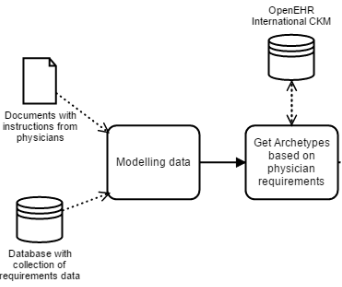
\includegraphics[width=0.465\textwidth]{img/LC_ARCH.PNG}
	\caption{Initial phase of archetype creation, using the example of openEHR CKM as a clinical models repository}
	\label{fig:LC_ARCH}
\end{figure}

Like all the others IT development projects, the final stage is the maintenance. After an archetype being published, is necessary to support it and continue to provide a continuous improvement on these artefacts. There are many reasons to keep maintenance, for instance, more additions could be implemented to the archetype that may reply to more specifications or requests from the vendors or the end users, some errors or bugs could be found and need to be quickly solved or could even be necessary to make a specialization using the parent archetype. Also after an archetype being published, its phase can constantly change. If this archetype gets a major or better version, it can be replaced, turning into an obsolete archetype. \\

It is really necessary that all these procedures should be carefully prepared with usual meetings with healthcare, IT and technical professionals to make sure that the final aim will be compliant with every side. Otherwise it can result in a creation of an archetype that does not met the specifications and turn on a waste of time by not being accepted on the openEHR CKM. Also, if it is possible to always send an english version of the submitted archetype, along with the translations of other languages, this could improve the time of revision, since the bigger part of the openEHR editor are english speakers. \\

For template creation, it does not need to have the same amount of work and preparation to get specific requirements and further development, comparing with the case of the archetype, since it is only an aggregation of a set of archetypes. \\

In the figure \ref{fig:arch_auth}, is possible to see the diagram made by the openEHR team \citep{Leslie2008} that currently takes care of the openEHR artefacts governance under the international CKM. The different archetype lifecycles are represented by the yellow boxes (draft, team review, published and obsolete) and those divide the different procedures made within each phase. 


\begin{figure}[H]
	\centering
    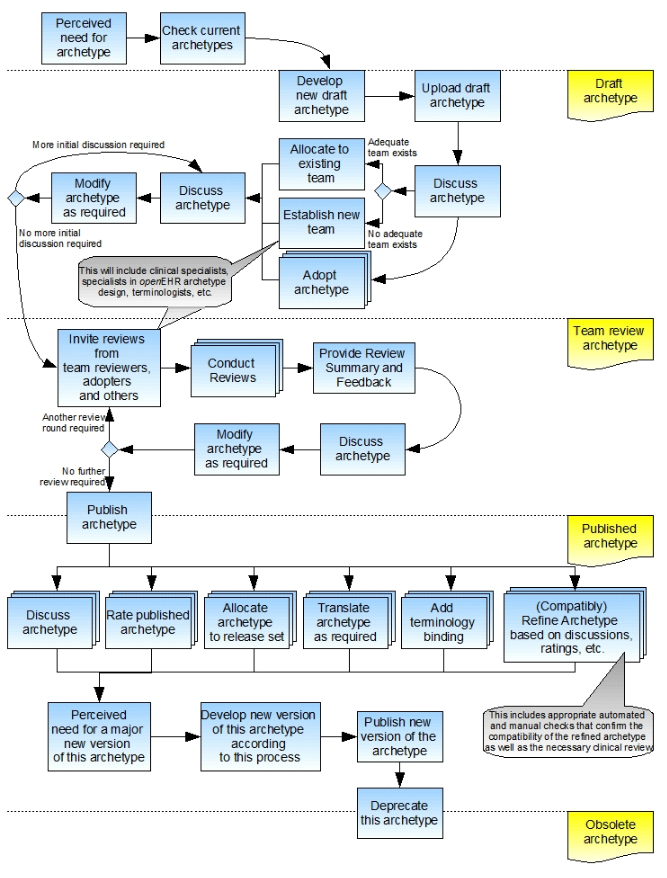
\includegraphics[width=0.815\textwidth]{img/arch_auth.PNG}
	\caption{Archetype authoring, review and publication \citep{Leslie2008}}
	\label{fig:arch_auth}
\end{figure}




\section{Distributed governance of archetypes}

The creation of an archetype usually starts when a need is found or a request is made, which will require a an openEHR modeler to start to construct it on his own computer alone or with a team from some project. This means that this archetype will have no custodial organization (e.g. au.gov.nehta, uk.org.clinicalmodels or org.openehr) managing it, getting the v0 version, following the \textit{semVer} rules, and the life cycle identifies it as "unmanaged" - this cycle does not exist on the openEHR CKM \citep{openehrckmgover2018}. After following all the steps described in the previous sub-chapter, when the archetype is done and prepared to be submitted to some ckm instance, it needs an approval from the custodian organization that manages that instance. After being submitted and accepted by the custodian organization, it gets this custodian name in the ARCHETYPE HRID namespace, e.g. \textbf{org.openehr::}openEHR-EHR-OBSERVATION.blood\_pressure.v1.adl and a new meta-data parameter within the archetype is filled as  e.g. ["custodian\_namespace"] = <"\textbf{org.openehr}"> along with a new UUID, license and copyright. Relatively to the versioning number, the major version is reset to 0 and the other versioning parameters (minor version and path) to 0.0.1. 

\begin{figure}[H]
	\centering
    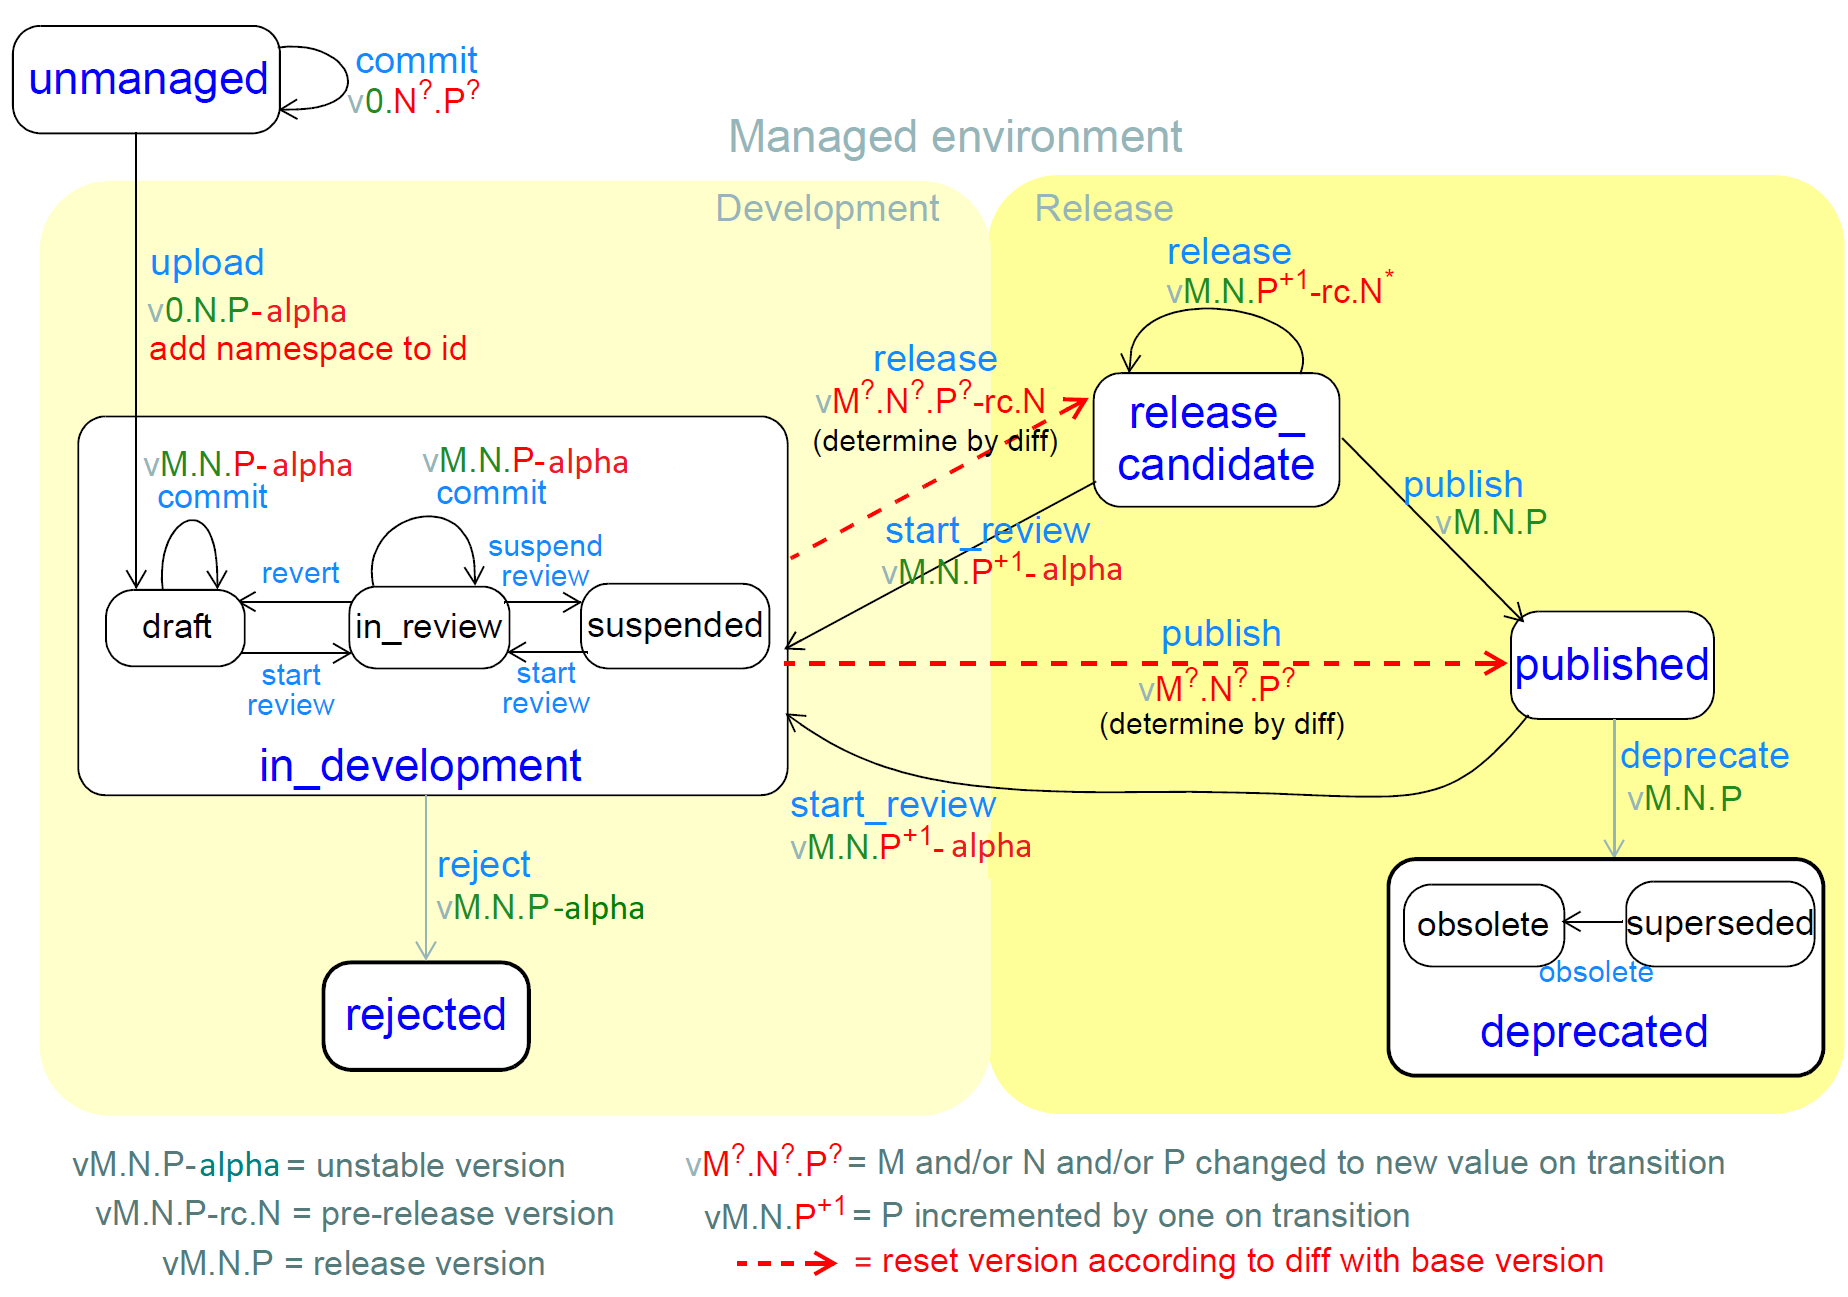
\includegraphics[width=1\textwidth]{img/development_lifecycle_with_versioning.png}
	\caption{Development Lifecycle with Versioning \citep{openehrckmgover22018}}
	\label{fig:development_lifecycle_with_versioning}
\end{figure}

Although an artefact can be accepted by a custodian organization, if this resource does not get an active maintenance, it can be rejected or migrated to another custodian organization. When this happens, the new custodian organization is allowed to make some changes on the archetype identification (human or machine readable way) under certain rules. In case of the human readable way, the \textit{namespace} can change to include the new organization, the \textit{concept\_id} (e.g. blood\_pressure) can also change depending on the new custodian requirements and the versioning parameter is usually changed to 0 (0.0.1). Since the human readable identifier (HRID) is changed, its \textit{uid} will be changed also to a new one, in conformity to the new name. Inside of the archetype content, there is a section to show the management history of an archetype that is being transfered between custodian organizations as it can be seen in table \ref{tab:arch_co_h}:

\begin{table}[H]
\caption{Archetype custodian organization history \citep{openehrckmgover2018}}
\label{tab:arch_co_h}
\centering
\begin{tabular}{l}
\toprule[2pt]
\begin{lstlisting}[language=XML]
    id_history = <
        ["2001-05-27"] = <
            old = <
                hrid = <"au.com.rbh::openEHR-EHR-EVALUATION.problem_desc.v2.4.1">
                uid = <"5221C9E5-0ECA-469F-83C5-A5D5A0C6682C">
            >
            new = <
                hrid = <"au.gov.nehta::openEHR-EHR-EVALUATION.problem.v1.0.1">
                uid = <"094C8B37-F0CD-45C9-A1B7-CDFDE14C67AB">
            >
        >
\end{lstlisting}
\tabularnewline \bottomrule[2pt]
\end{tabular}
\end{table}


\newpage
\section{Governance of a local repository based on openEHR artifacts}

This section presents a recommendation by the author. The available information about this topic on scientific jornals or articles is minimal or almost inexistent and not directed to the openEHR artifacts, but to software coding in general. \\

When new EHR project based on openEHR standards have the specifications and requirements phase are already prepared and ready to get the development phase with the artifacts, the gathered information needs to be stored and always updated when necessary. The openEHR resources are not statical, a lot of new updates are made constantly to improve the knowledge saved and retrieved from them. The best way is to construct a local CKM, that needs to be compliant with the openEHR CKM, as explained in the previous chapters. \\ 

Maintaining a repository based on openEHR compliant with the openEHR CKM can be hard and time consuming if not wrought since the beginning of its creation. Sometimes different modelers or even programmers created and changed the archetypes in such a away, that is complicated in a case of a new person on charge to take care of the CKM repository. If this repository is not managed in a way to care of the content and changes of these resources, which are what keep and structure the most important part of an EHR system, the health data, the repository can end up in a imbroglio of misleading data structures. \\

For that, the following steps should help to maintain, in a better way, the management of a local CKM: 
\begin{enumerate}
\item Choose a person responsible to create and maintain the repository. A person with a background in engineering or informatics with knowledge of medical concepts and that have been study the openEHR specification, suits the best. A "backup" responsible can also be a good choice to do not all the repository knowledge imprisoned to just one person, just in case.
\item When creating a new CKM repository to store the openEHR artifacts that have been downloaded from the openEHR CKM, a good choice is to use one that supports \ac{CVS} and is hosted online. As a personal choice, if the enterprise or company where the project that will depend from artifacts has a GitLab instance, use that instance, if not, use GitHub. Both are free to use and offer a good support. Hereupon is possible to maintain a creation and edition history of those artifacts. If there are archetypes saved on a local computer that are being used on current projects, but not available online, that knowledge can be easily lost. \ac{SVN} based repositories are also complicated to maintain on large projects, so it should not be a valid choice. 
\item Choose a openEHR archetype and template editor. As a personal choice, the ADL Designer web-tool is user-friendly, free to use and is the most supported nowadays. Also it offer connection to the local repository and commit the changes made to it.  
\item The responsible person should be on charge of making weekly verification updates from the local openEHR resources with the ones available from the openEHR CKM. Using the script created from this dissertation can help (note: only if the local repository is connected to the ADL Designer tool). 
\item In case of finding an archetype that needs to be updated, prepare time to check and change all the templates that also make use of this resource. Sometimes adding terminology to the template needs to be done again, among others.
\item The responsible person of the local repository should have an active testing of the forms used within the developing project. An error related with archetypes may arise and since the responsible has an openEHR experience, he would know how to solve it quickly. Also all the existent combinations that can be done on the form should be tested before deployment, and this can be time consuming. If a bug is found due to a mistake on the archetype logic, report it immediately to the openEHR CKM page, for correction and further update. It is important to remember that these archetypes live through an active community that works for free to correct some bug in these artifacts. Do not forget that a bug in the archetype of your project can exist in other projects that are using the same archetype. Communication and reporting is the golden standard for local and international improvement of the openEHR standard.
\item If a new requirement requires a new archetype, search if there is some created resources in the openEHR CKM. Use specific keywords to search your subject, choose the archetype and read the associated header along with the use and misuse of this resource. A lot of new archetypes are created inside of local repositories due to a poor search on openEHR CKM. If the openEHR CKM has your topic, but does not include everything you want, suggest a new review to include your content, or specialize the one you want. Nevertheless, send your new archetype for review on the openEHR CKM. A lot of content is being created and reviewed and new clinical content to enrich this platform is always welcome. 
\item If you create a new archetype to fit local requirements, do not name it with the same name as the other archetypes on openEHR CKM and use a correct lifecycle for the process of archetype creation. OpenEHR has very well defined parameters of how to deal with this topic that were mentioned in the previous chapters.

\end{enumerate}

Following these steps, can help to lead on good governance of the openEHR resources from the local CKM repositories. But this just depends on how the company and the project manager knows the value of having this data knowledge updated and put on charge a responsible for this task. A lot of projects that does not have any governance of their repositories, ended up with a jumble of information on the databases which is almost impossible to correct in a proper way,  due to the time consuming that this task can be. If the local CKM repository is created and maintained in a proper way since the begging, the constant updating of resources would take between one to two hours per week for correction, or even less, depending on how much templates are connected to the updated archetypes.  

\end{document}